\section{Main results}
Let $\fp\in\Sn$ be a permutation. For simplicity (cf. \cref{sec:fixed_pts}), we assume that $\fp$ has no fixed points, i.e.  $\fp(i)\neq i$ for all $i\in[\n]:=\{1,2,\dots,\n\}$. 
 %

\begin{figure}
\begin{tabular}{cccc}
\includegraphics[width=0.13\textwidth]{figures/L4a1} &
\includegraphics[width=0.27\textwidth]{figures/Lperm} &
\includegraphics[width=0.24\textwidth]{figures/Ltor}&
\hspace{0.05in}\includegraphics[width=0.25\textwidth]{figures/Ltor_emb}\\
  (a) \linkurl{L4a1} & (b) $\Lperm_\pi$ & (c) $\Ltor_\pi$ & (d) \hspace{0.05in}$\T\hookrightarrow\R^3$
\end{tabular}
%
%
%
%
%
%
  \caption{\label{fig:L4a1} The links \linkurl{L4a1}$\cong \Lperm_\pi\cong\Ltor_\pi$ for $\pi$ given by~\eqref{eq:intro:fp}.}
\end{figure}


In~\cite{GL_qtcat}, we described a way to associate a \emph{positroid link} $L_\fp$ to such $\fp$. The number of components of $L_\fp$ is given by the number $\ncyc(\fp)$ of cycles of $\fp$. Our running example will be
\begin{equation}\label{eq:intro:fp}
 \fp=\left(\!\!\text{
\begin{tabular}{cccccccc}
\textcolor{red}{$1$} & \textcolor{blue}{$2$} & \textcolor{blue}{$3$} & \textcolor{red}{$4$} & \textcolor{red}{$5$} & \textcolor{blue}{$6$} & \textcolor{blue}{$7$} & \textcolor{blue}{$8$}\\
\textcolor{red}{$4$} & \textcolor{blue}{$6$} & \textcolor{blue}{$8$} & \textcolor{red}{$5$} & \textcolor{red}{$1$} & \textcolor{blue}{$3$} & \textcolor{blue}{$2$} & \textcolor{blue}{$7$}
\end{tabular}
}\!\!\right),
\end{equation}
written in two-line notation, with different colors representing different cycles of $\fp$. We have $\n=8$ and $\ncyc(\fp)=2$. The associated positroid link $L_\fp$ is shown in \figref{fig:L4a1}(a); it appears under the name \linkurl{L4a1} in the Thistlethwaite Link Table~\cite{KAT}. 

\subsection{Positroid links} \label{sec:intro:positroid_links}

Our first result relates several different representations of the link $L_\fp$, confirming the conjectures of~\cite{GL_qtcat,GL_cat_combin}. We start by giving a brief overview of these descriptions; see \cref{sec:positr-comb,sec:positr-link-isot} for full details.

\subsubsection{Permutation link} \label{sec:intro:perm_links}
Draw $\n$ points labeled $1,2,\dots,\n$ on the circle in clockwise order. Draw a line segment connecting $i$ to $\fp(i)$, for each $i\in[\n]:=\{1,2,\dots,\n\}$. If two line segments $[i, \fp(i)]$, $[j,\fp(j)]$ cross for some $i,j\in[\n]$ such that $\fp(i)<\fp(j)$, then the segment $[j,\fp(j)]$ is drawn above $[i, \fp(i)]$; see \figref{fig:L4a1}(b). 
%
 The union of these segments gives rise to a link diagram. We refer to the resulting link as the \emph{permutation link} of $\fp$, denoted $\Lperm_\fp$. Orienting each line segment from $i$ to $\fp(i)$ induces an orientation on $\Lperm_\fp$.


\subsubsection{Toric permutation link}\label{sec:intro:tor_links} Let $\T:=\R^2/\Z^2$ be the torus. Consider its fundamental domain $[0,1]^2$ which we view as a square subdivided into $\n^2$ boxes of size $\frac1\n\times \frac1\n$. We denote by $b_{i,j}$, $1\leq i,j\leq \n$, the box whose upper right corner has coordinates $\frac1\n(i,j)$. For each $i\in[\n]$, place a dot $d_i$ in box $b_{i,\n+1-i}$. Draw an arrow (in $\T$) in the northeast direction from $d_i$ to $d_{\fp(i)}$ for each $i\in[\n]$. When two such arrows cross, the arrow with the higher slope is drawn above the arrow with the lower slope. We obtain a planar diagram of an oriented link $\Ltor_\fp$ drawn on the surface of $\T$; see \figref{fig:L4a1}(c). Any link drawn on $\T$ may be converted into a link in $\R^3$ using the procedure shown in \figref{fig:L4a1}(d). Abusing notation, we denote by $\Ltor_\fp$ the resulting link in $\R^3$.

\begin{remark}
Viewing $\Ltor_\fp$ as drawn on the surface of $\T$ (resp. in a solid torus $S^1\times [0,1]^2$) contains more information---it gives rise to a certain elliptic Hall algebra element~\cite{ScVa,BuSc} (resp. to a symmetric 
%
function~\cite{Turaev}) with deep connections to Khovanov--Rozansky homology. We aim to pursue this direction in an upcoming paper~\cite{GL_EHA}.
\end{remark}
%
%


\begin{figure}
  \includegraphics[width=1.0\textwidth]{figures/grid_iso}
  %
 \caption{\label{fig:grid_iso} Toric grid links; see \cref{rmk:grid} and \cref{sec:perm-to-toric}.}
\end{figure}


\begin{remark}\label{rmk:grid}
We may also view $\Ltor_\fp$ as coming from a \emph{grid diagram} (see e.g.~\cite{OSS}). The grid diagram of $\fp$ is obtained by placing an $X$ in box $b_{i,\n+1-i}$ and an $O$ in box $b_{i,\n+1-\fp(i)}$ for each $i\in[\n]$. We then connect the $X$'s and the $O$'s by horizontal and vertical segments, always drawing the vertical segments above the horizontal ones. More precisely, to a given grid diagram, we can associate two links. First, a \emph{toric grid link} $\Lgridt_\pi$, drawn on the surface of $\T$, is obtained by drawing a horizontal arrow from $O$ to $X$ pointing right in each row, and a vertical arrow from $X$ to $O$ pointing up in each column; see \figref{fig:grid_iso}(b). (In \cref{fig:grid_iso}, for each $i\in[\n]$, we place an $i$ instead of an $X$ in box $b_{i,\n+1-i}$.) Second, a \emph{planar grid link} $\Lgrid_\pi$, whose planar diagram is drawn inside $[0,1]^2$, is obtained by drawing a horizontal arrow from $O$ to $X$ in each row, and a vertical arrow from $X$ to $O$ in each column, but in this case the arrows are not allowed to cross the boundaries of $[0,1]^2$; see \figref{fig:grid_iso}(c). As explained in~\cite[Section~3.2]{OSS}, these two links are isotopic to each other. It is easy to see that the toric grid link $\Lgridt_\pi$ is also isotopic to $\Ltor_\fp$.
\end{remark}

%


\begin{figure}
  \includegraphics[width=1.0\textwidth]{figures/Lrich}
  \caption{\label{fig:Lrich} A Richardson braid (left) and a Richardson link (right) defined in \cref{sec:intro:Rich_link}.}
\end{figure}


\subsubsection{Richardson link}\label{sec:intro:Rich_link} A permutation $w\in\Sn$ is called \emph{$k$-Grassmannian} if $w(1)<\cdots<w(\n-k)$ and $w(\n-k+1)<\cdots<w(\n)$. We denote by $\Skn$ the set of $k$-Grassmannian permutations. The permutation $\fp$ can be uniquely decomposed as the product $\fp=wv^{-1}$ for some $1\leq k\leq \n-1$ and some pair $(v,w)\in \Sn\times\Skn$ such that $v\leq w$ in the Bruhat order on~$\Sn$; see \cref{cor:KLS}. For the permutation $\fp$ given by~\eqref{eq:intro:fp}, we get that $k=4$ and\footnote{Our convention for multiplying permutations is right-to-left, i.e.  $\fp(j)=w(v^{-1}(j))$ for all $j\in[\n]$.}
\begin{equation*}%
v=\left(\!\!\text{
\begin{tabular}{cccccccc}
\textcolor{red}{$1$} & \textcolor{red}{$2$} & \textcolor{blue}{$3$} & \textcolor{blue}{$4$} & \textcolor{red}{$5$} & \textcolor{blue}{$6$} & \textcolor{blue}{$7$} & \textcolor{blue}{$8$}\\
\textcolor{red}{$1$} & \textcolor{red}{$4$} & \textcolor{blue}{$2$} & \textcolor{blue}{$3$} & \textcolor{red}{$5$} & \textcolor{blue}{$7$} & \textcolor{blue}{$6$} & \textcolor{blue}{$8$}
\end{tabular}
}\!\!\right)
,\quad
w=\left(\!\!\text{
\begin{tabular}{cccccccc}
\textcolor{red}{$1$} & \textcolor{red}{$2$} & \textcolor{blue}{$3$} & \textcolor{blue}{$4$} & \textcolor{red}{$5$} & \textcolor{blue}{$6$} & \textcolor{blue}{$7$} & \textcolor{blue}{$8$}\\
\textcolor{red}{$4$} & \textcolor{red}{$5$} & \textcolor{blue}{$6$} & \textcolor{blue}{$8$} & \textcolor{red}{$1$} & \textcolor{blue}{$2$} & \textcolor{blue}{$3$} & \textcolor{blue}{$7$}
\end{tabular}
}\!\!\right)
.
\end{equation*}
%
Here, the colors represent the cycles of $\fp=wv^{-1}$. 
 Let $\beta(v),\beta(w)$ be the positive braid lifts of $v,w$ to the braid group of $\Sn$. Consider the \emph{Richardson braid} $\beta_{v,w}:=\beta(w)\cdot \beta(v)^{-1}$ shown in \figref{fig:Lrich}(left). Taking the \emph{braid closure} of $\beta_{v,w}$, we obtain the \emph{Richardson link} $\Lrich_{v,w}=\Lrich_\fp$ shown in \figref{fig:Lrich}(right). We orient the strands of $\beta_{v,w}$ from right to left; cf. \figref{fig:Lrich-to-L'}(left).
%
\begin{remark}\label{rmk:Rich_Young}
It is well known (cf. \cref{sec:Le-diags}) that $k$-Grassmannian permutations are in bijection with Young diagrams that fit inside a $k\times (\n-k)$ rectangle. Thus, in \figref{fig:Lrich}(left), we arrange the crossings in $\beta(w)$ into a (rotated) Young diagram. The condition that $v\leq w$ in the Bruhat order implies that a reduced word for $v$ is a subword of a reduced word for $w$, and thus we represent $\beta(v)^{-1}$ in \figref{fig:Lrich}(left) by replacing some of the crossings in $\beta(w)^{-1}$ with ``elbows.''
%
\end{remark}

 The above recipe was used in~\cite{GL_qtcat} more generally for pairs $v\leq w$ where $w$ is not necessarily $k$-Grassmannian. 

\begin{figure}
\includegraphics[width=1.0\textwidth]{figures/Lplab}
  \caption{\label{fig:Lplab} Converting a plabic graph $G$ into the plabic graph link $\Lplab_G$.}
\end{figure}


\subsubsection{Plabic link} \label{sec:intro:plabic_link}
%
A \emph{plabic graph} is a non-empty planar graph $G$ embedded in a disk with vertices colored black and white; see~\cite{Pos}.  
%
 A \emph{strand} in $G$ is a path that makes a sharp right turn at each black vertex and a sharp left turn at each white vertex. We assume that the graph $G$ has $\n$ boundary vertices, all of which have degree $1$ and are labeled $1,2,\dots,\n$ in clockwise order. An example of a plabic graph $G$ is shown in \figref{fig:Lplab}(a), and the strands in $G$ are shown in \figref{fig:Lplab}(b).

The following description of the \emph{plabic graph link} $\Lplab_G$, or \emph{plabic link} for short, can be deduced from~\cite{ACampo,STWZ,FPST} by breaking the symmetry following~\cite{Hirasawa}. (See \cref{sec:plabic_links_properties} for a more invariant description.) The planar diagram of $\Lplab_G$ will consist of the union of the strands of $G$. To specify the overcrossings, let $p$ be an intersection point of two strands $S_1,S_2$ in $G$.  The tangent vector to $S_1$ (resp. $S_2$) at $p$ can be considered a vector in the complex plane, and we let $\Arg(S_1,p) \in[0,2\pi)$ (resp. $\Arg(S_2,p)\in[0,2\pi)$) denote the argument of this vector.
%
We assume that $0<\Arg(S_1,p)\neq\Arg(S_2,p)<2\pi$. Then $S_1$ is drawn above $S_2$ if $\Arg(S_2,p)>\Arg(S_1,p)$, otherwise $S_1$ is drawn below $S_2$. 

\begin{figure}
\includegraphics[width=0.7\textwidth]{figures/over_under}
  \caption{\label{fig:over_under} For every point $p$ on a strand $S$ satisfying $\Arg(S,p)=0$, we insert a strand segment going to the boundary and back; see \cref{sec:intro:plabic_link}.}
\end{figure}



A technical extra step is required to finalize the construction of $\Lplab_G$; see \cref{fig:over_under}. Consider a point $p$ on a strand $S$ such that $\Arg(S,p)=0$, i.e.  such that $S$ is directed to the right at $p$. We add an extra segment $S'$ to $S$ traveling from $p$ to the boundary of the disk followed by a segment $S''$ traveling from the boundary back to $p$. In the neighborhood of $p$, $S$ looks like a plot of a function. If this function is ``concave up'' at $p$ (i.e.  has positive second derivative), then $S'$ (resp. $S''$) is drawn below (resp. above) all other strands. If $S$ is ``concave down'' at $p$ then $S'$ (resp. $S''$) is drawn above (resp. below) all other strands. 

Finally, each boundary vertex of $G$ is an endpoint of exactly two strands (one outgoing and one incoming). We join these endpoints together and obtain a planar diagram of a link denoted $\Lplab_G$. See \figref{fig:Lplab}(c), where the points $p$ such that $\Arg(S,p)=0$ are marked by the symbol $\mysq$.

 The strands in $G$ that start and end at the boundary vertices give rise to the \emph{strand permutation} $\pig$ of $G$. In this subsection, we will assume that $G$ is \emph{reduced}, i.e.  that $G$ has the minimal possible number of faces among all graphs with a given strand permutation. Importantly, in \cref{sec:intro:quivers-point-count}, we will drop this assumption. Postnikov~\cite{Pos} showed that for any $\pi\in \Sn$, there exists a reduced plabic graph $G$ with strand permutation $\pig=\pi$. For example, for $\pi$ given by~\eqref{eq:intro:fp}, one can take $G$ to be the graph in \figref{fig:Lplab}(a). Up to isotopy, the resulting link $\Lplab_G$ depends only on $\pi$ and is denoted $\Lplab_\pi$. 

%
%
%

%


%
%


\begin{figure}
\includegraphics[width=1.0\textwidth]{figures/concave_1}
  \caption{\label{fig:concave} Converting a concave curve $C$ into the link $\Ltor_{\pi_C}$ for some $\pi_C\in\Sn$; see \cref{ex:intro:Cox}.}
\end{figure}


\subsubsection{Coxeter link} \label{sec:intro:cox_link}
In~\cite[Section~6]{GL_cat_combin}, we studied \emph{concave permutations}, defined as follows. Choose a generic concave curve $C$ inside a $k\times (\n-k)$ rectangle connecting $(0,0)$ to $(\n-k,k)$ as in \figref{fig:concave}(a). We will shift it by the vector $(-\eps,\eps)$ for some small $\eps>0$ as in \figref{fig:concave}(b). Under the natural projection $\R^2\to\T=\R^2/\Z^2$, the curve $C+(-\eps,\eps)$ projects to a curve $\Cproj$ in the unit square $[0,1]^2$. For each self-intersection of $\Cproj$, we draw the segment of the higher slope above the segment of the lower slope; see \figref{fig:concave}(c). The resulting link diagram is isotopic to $\Ltor_\pi$ for a permutation $\pi=\pi_C\in\Sn$ which can be explicitly read off from $\Cproj$ as follows. Label the intersection points of $\Cproj$ with the $y=1-x$ diagonal of $[0,1]^2$ by $d_1,d_2,\dots,d_\n$, proceeding in the northwest direction. Thus, $d_1=(1-\eps,\eps)$ is the projection of the starting and ending points of $C+(-\eps,\eps)$. In \figref{fig:concave}(c), we represent each point $d_i$ by~$i$. Since $C$ was generic, we assume that the points $d_1,d_2,\dots, d_\n$ are pairwise distinct. The permutation $\pi_C$ is defined so that each segment of $C$ connects (in the northeast direction) $d_i$ to $d_{\pi(i)}$ for some $i\in[\n]$. See \figref{fig:concave}(d). We refer to permutations that can be obtained in this way as \emph{concave permutations}. They form a subclass of the class of \emph{repetition-free permutations} introduced in~\cite{GL_cat_combin}.

Let $\la_C=(\la_1,\la_2,\dots,\la_k)$ be the Young diagram inside the $k\times (\n-k)$ rectangle consisting of all unit boxes strictly above $C$, shown in \figref{fig:concave}(a). 
%
 Consider a sequence $\abf(C)=(a_2,\dots,a_k)$ given by $a_i:=\la_{i-1}-\la_i$ for $2\leq i\leq k$. The \emph{Coxeter link} $\Lcox_C$ is the closure of the braid
\begin{equation}\label{eq:beta_abf_dfn}
  \beta(\abf(C)):=\ell_2^{a_2}\cdots \ell_k^{a_k}\cdot\sigma_1\cdots \sigma_{k-1},
\end{equation}
where $\sigma_1,\dots,\sigma_{k-1}$ are the standard braid group generators of the braid group of $S_k$, and $\ell_i=\sigma_{i-1}\cdots \sigma_1\cdot \sigma_1\cdots \sigma_{i-1}$ are the Jucys--Murphy elements. 

\begin{figure}
\includegraphics[width=0.85\textwidth]{figures/concave_2}
  \caption{\label{fig:concave_2} Converting a concave curve $C$ into the Coxeter braid $\beta(\abf(C))$.}
\end{figure}
\begin{example}\label{ex:intro:Cox}
Let $C$ be the curve shown in \cref{fig:concave,fig:concave_2}. We have $k=5$ and $\n=9$. The permutation $\pi_C=\left(\!\!\text{
\begin{tabular}{ccccccccc}
%
%
$1$ & $2$ & $3$ & $4$ & $5$ & $6$ & $7$ & $8$ & $9$\\
$6$ & $8$ & $7$ & $9$ & $2$ & $4$ & $1$ & $3$ & $5$
\end{tabular}
}\!\!\right)$ can be read off from the labels\footnote{The labels in \figref{fig:concave}(b) are chosen in such a way that when we project $C$ to the unit square, they become ordered along the diagonal $y=1-x$; see \figref{fig:concave}(c).} in \figref{fig:concave}(b): in cycle notation, $\pi_C$ is given by $\pi_C=(1\,6\,4\,9\,5\,2\,8\,3\,7\,1)$. We have $\la_C=(2,1,1,0,0)$, $\abf(C)=(1,0,1,0)$,  and $\beta(\abf(C))=\ell_2\ell_4\sigma_1\sigma_2\sigma_3\sigma_4$; see also~\cite[Figure~13]{GL_cat_combin}.
\end{example}
%
 Coxeter links and their Khovanov--Rozansky homology have previously been studied in relation to flag Hilbert schemes and generalized shuffle conjectures~\cite{ObRo,GN,GNR,BHMPS}; see also~\cite[Section~7.2]{GL_cat_combin}.
%
 %
%
%

The following is our first main result.
\begin{theorem}\label{thm:isotopy}
  Let $\fp\in\Sn$ be a permutation without fixed points. Then the links $\Lperm_\fp$, $\Ltor_\fp$, $\Lrich_\fp$, and $\Lplab_\fp$ are all isotopic. If $\fp=\fp_C$ for some concave curve $C$ then each of these links is also isotopic to $\Lcox_C$.
%
\end{theorem}
We refer to any one of the above links as the \emph{positroid link} of $\fp$.

%
%
%

%

%


\begin{remark}
The recent work~\cite{CGGS} independently constructs Legendrian isotopies (a stronger result than our smooth isotopies) between the Richardson link $\Lrich_\pi$ and other closely related links: closures of juggling braids, cyclic rank matrix braids, and Le-diagram braids.  We expect the Le-diagram braid in~\cite{CGGS} to be closely related to our plabic graph link $\Lplab_\fp$, and the juggling braid to be similar to our permutation link $\Lperm_\fp$, though we believe our definition of $\Lperm_\fp$ is the simplest and most elementary.

Isotopies between cyclic rank matrix links and plabic graph links have also been observed in~\cite{STWZ}.
%
%
\end{remark}

\subsection{Quiver point count and the HOMFLY polynomial}\label{sec:intro:quivers-point-count}
In this subsection, we consider not necessarily reduced plabic graphs $G$. Throughout the paper, we assume that the interior faces of $G$ are simply connected, i.e.  that no interior face of $G$ contains another connected component of $G$ inside of it. For simplicity, we also assume that each plabic graph $G$ is \emph{trivalent}, i.e.  that each interior vertex of $G$ has degree $3$. (Recall that the boundary vertices of $G$ are always required to have degree $1$.) This is not a restrictive assumption: any vertex of degree $2$ in $G$ can be omitted (joining two of its neighbors by an edge), and any vertex of degree higher than $3$ in $G$ can be ``uncontracted'' into several vertices of degree $3$ of the same color; see~\cite[Figure~12.2]{Pos}.
%
%
%
%

Let $G$ be a (trivalent) plabic graph. The planar dual of $G$ naturally contains a directed (sub)graph denoted $\QG$. Explicitly, place a vertex of $\QG$ inside each \emph{interior face} of $G$ (i.e.  a face not incident to the boundary of the disk). For every edge $e$ of $G$ whose endpoints are of different color and such that the two faces $F,F'$ incident to $e$ are both interior, $\QG$ contains an arrow between $F$ and $F'$. (These two faces $F,F'$ may or may not be equal.) The direction of the arrow is chosen so that the white endpoint of $e$ is on the left as one moves along this arrow. See \cref{fig:simple}.


\begin{figure}
  \includegraphics[width=1.0\textwidth]{figures/simple}
  \caption{\label{fig:simple} Examples of simple and non-simple plabic graphs $G$ (black) and the associated quivers $\QG$ (red).}
\end{figure}

%
 The following definition is crucial for our analysis.
\begin{definition}
A plabic graph $G$ is called \emph{simple} if the directed graph $\QG$ is a \emph{quiver}, i.e.  contains no directed cycles of length $1$ and $2$.
\end{definition}
For example, the plabic graph $G$ in \figref{fig:simple}(b) is not simple since $\QG$ contains a pair of opposite arrows. The graph $G$ in \figref{fig:simple}(d) is not simple since $\QG$ contains a loop arrow. The graphs in \figref{fig:simple}(a,c) are simple.
%

%

%


%

To every \emph{\Louise} quiver $Q$ (see~\cref{sec:quiver}), we associate a rational function $\RQ(q)$ called the \emph{point count rational function}. It can be computed via an explicit recurrence relation: see~\eqref{eq:RQ_recurrence} and~\eqref{eq:RQ_skein}. The function $\RQ(q)$ has the following interpretation in terms of \emph{cluster algebras}~\cite{FZ}; see~\cref{sec:quiver} for the relevant definitions. 
Let $Q$ be a quiver with $n$ vertices. Consider an ice quiver $\Qice$ with $m$ frozen vertices and mutable part $Q$, and assume that the rows of the $(n+m)\times n$ exchange matrix $\BQice$ of $\Qice$ span $\Z^n$ over $\Z$. Then the cluster algebra $\AQice$ gives rise to a \emph{cluster variety} $\XQice$, and its point count over a finite field $\F_q$ with $q$ elements (for $q$ a prime power) is given by
\begin{equation*}%
  \#\XQice(\F_q)=(q-1)^m\cdot \RQ(q);
\end{equation*}
see \cref{prop:Q_pcnt}.

%
%

 A typical example of this phenomenon occurs when $G$ is a reduced plabic graph: then, by~\cite{GL_cluster}, 
 %
%
  $\AQGice$ is the coordinate ring of the associated \emph{open positroid variety} $\Pio_G$ inside the Grassmannian~\cite{Pos,KLS}. In particular, $(q-1)^{\n-\conn(G)}\RQG(q)$ counts the number of points in $\Pio_G(\F_q)$, where $\n$ is the number of boundary vertices of $G$ and $\conn(G)$ is the number of connected components of $G$.%

Given an (oriented) link $L$, one can define a Laurent polynomial $\HOMP(L)=\HOMP(L;a,z)$ called the \emph{\FLY polynomial}~\cite{HOMFLY,PT} of $L$. It is defined by the skein relation
\begin{equation}\label{eq:HOMFLY_dfn}
  %
  a\HOMP(L_+) - a^{-1} \HOMP(L_-)=z\HOMP(L_0)\quad \text{and}\quad \HOMP(\unknot)=1.
\end{equation}
Here, $\unknot$ denotes the unknot and  $L_+$, $L_-$, $L_0$ are any three links whose planar diagrams locally differ as  follows.
\newcommand\lw{3pt}
\newcommand\lww{10pt}
\newcommand\drcirc{
\draw[line width=0.3pt, dashed] (0,0) circle (1cm);
}
\newcommand\scl{0.4}

\newcommand\DA{30}
\begin{center}
\begin{tabular}{ccc}
\scalebox{\scl}{
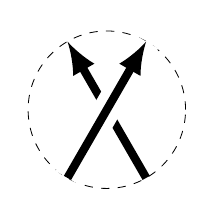
\begin{tikzpicture}
\drcirc
\draw[line width=\lw,->,>=latex] (-90+\DA:1)--(90+\DA:1);
\draw[line width=\lww,white] (-90-\DA:1)--(90-\DA:1);
\draw[line width=\lw,->,>=latex] (-90-\DA:1)--(90-\DA:1);
\end{tikzpicture}
} 

& 

 
\scalebox{\scl}{ 
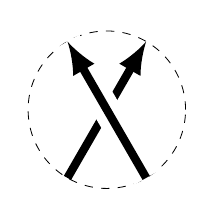
\begin{tikzpicture}
\drcirc
\draw[line width=\lw,->,>=latex] (-90-\DA:1)--(90-\DA:1);
\draw[line width=\lww,white] (-90+\DA:1)--(90+\DA:1);
\draw[line width=\lw,->,>=latex] (-90+\DA:1)--(90+\DA:1);
\end{tikzpicture} 
} 
& 
 
\newcommand\rc{10} 
\scalebox{\scl}{ 
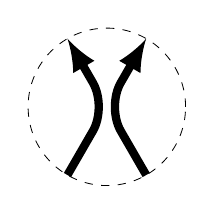
\begin{tikzpicture}
\drcirc
\draw[line width=\lw,->,>=latex,rounded corners=\rc] (-90-\DA:1)--(0,0)--(90+\DA:1);
\draw[line width=\lw,->,>=latex,rounded corners=\rc] (-90+\DA:1)--(0,0)--(90-\DA:1);
\end{tikzpicture} 
} 
\\ 
$L_+$  &  $L_-$  &  $L_0$

  

\end{tabular}
\end{center}
